% Author: PokMan Ho
% Script: res.tex
% Desc: MRes thesis result section
% Input: none
% Output: none
% Arguments: 0
% Date: Jan 2020

\documentclass[../thesis.tex]{subfiles} %% use packages & commands as this main file

\begin{document}
\section{Result}
%% text on all result -> all graphs
From Table \ref{tab:eqm}, P-only systems (eqm 3) could not give a biologically meaningful result for ``no harvest" setting under the current set of model assumptions.  Hence comparisons between with/without harvest were only done for P+B systems (eqm 4).  Comparing with/without carbon harvest in P+B systems (Fig.\ref{fig:wilcox}), the effort was statistically higher than ``no harvest" scenario only when the harvest rate was larger than 8/day.  Hence the closest significant sampled harvest rate with ``harvest" $>$ ``no harvest" was 9/day (W=57407, p=0.011).  However out of 1100 samples drew via LHS, about 90\% (n=991, median = -0.0016 (4dp)) feasible scenarios for ``no harvest" setting but only 12\% (n=134, median = 0.5670 (4dp)) for $x=9$/day.  On the other hand, P+B systems with harvest was statistically higher than their P-only counterparts for harvest rates higher than 1/day (Fig.\ref{fig:wilcox}).  At the closest significant sampled harvest rate with P+B $>$ P-only systems (2/day; W=129849, p$\ll$0.01), all (n=1100, median = -1.1334 (4dp)) scenarios were feasible for P-only system while only 25\% (n=275, median = -0.5379 (4dp)) for the P+B setting.



Only P+B systems were able to compare the effect of with/without carbon harvest due to mathematical constraints in P-only systems (Table \ref{tab:eqm}).  Harvest rate of more than 1/day was 

\begin{figure}[H]
    \centering
    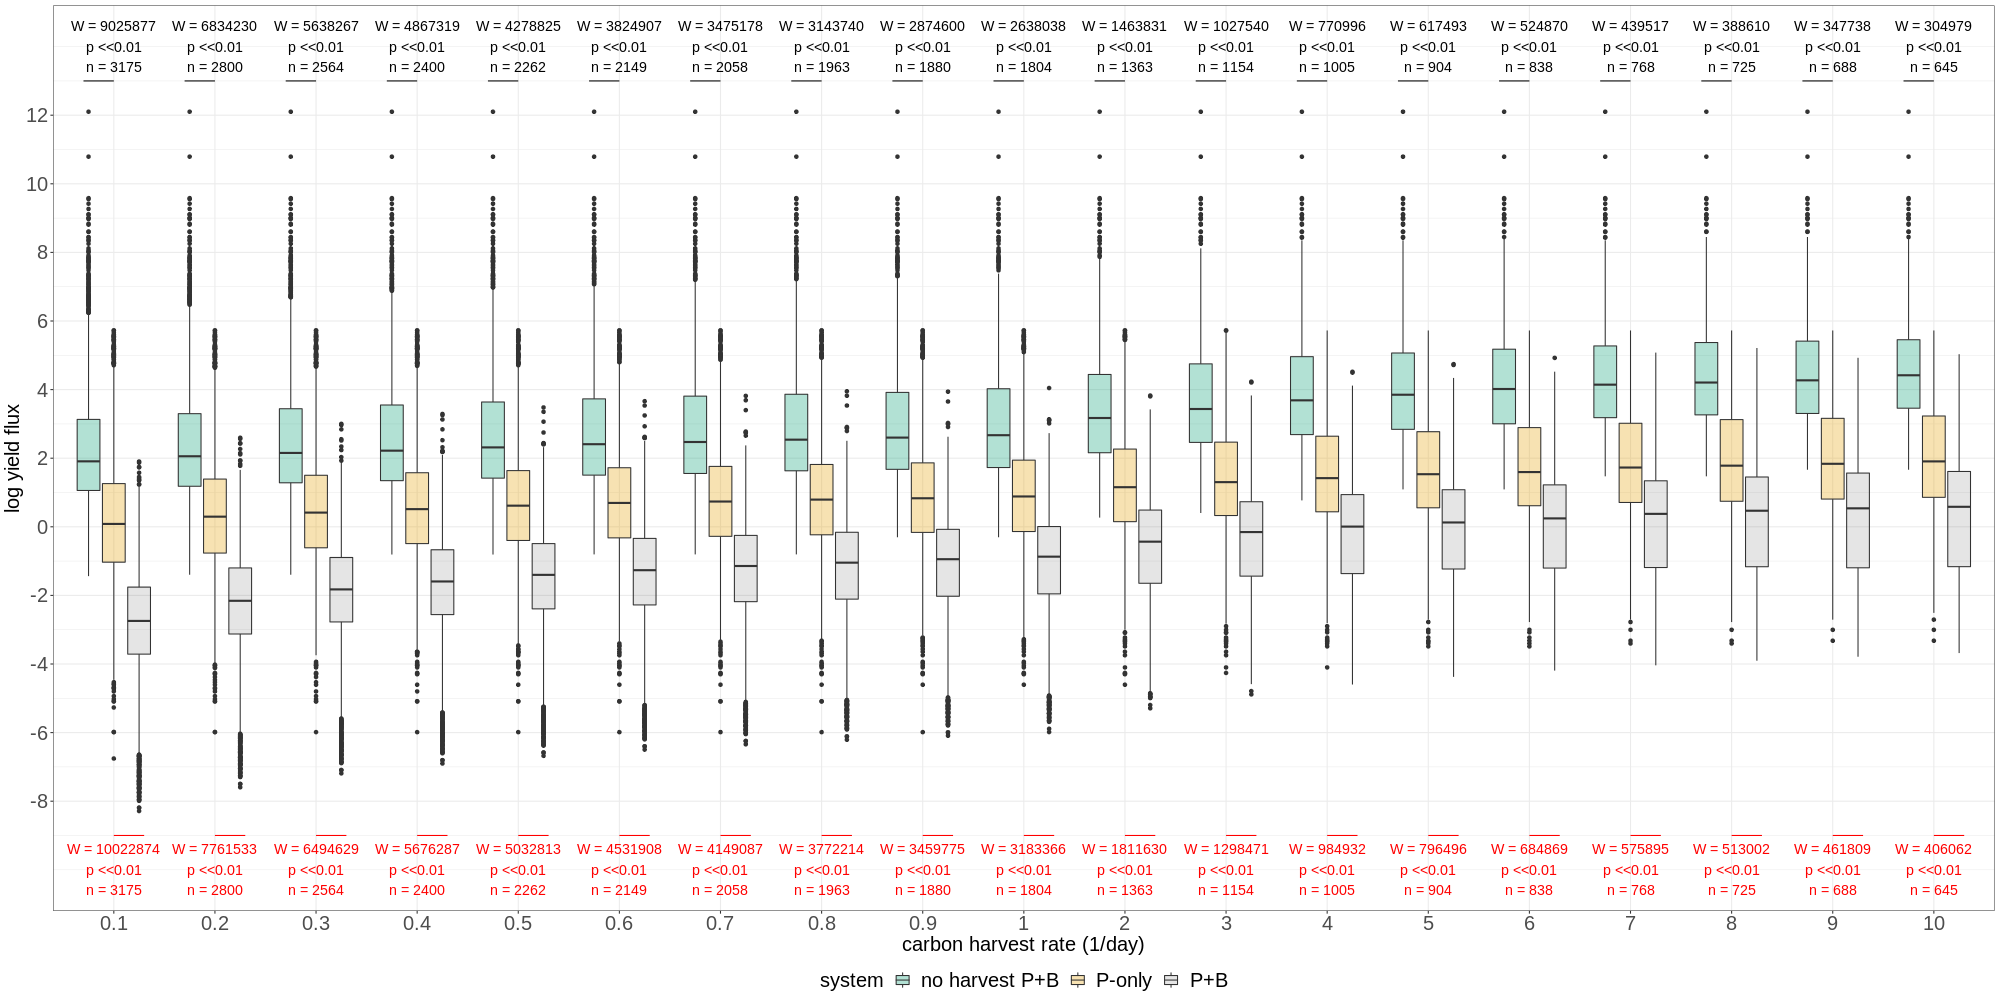
\includegraphics[width=\linewidth]{../result/Wilcox.png}
    \caption[Wilcox test summary]{Line graph showing Wilcox signed rank test (W-test) result (solid line) and respective p-values (dashed line) between P-only and P+B systems on ``log total carbon" and ``log yield flux" perspectives.  {\scriptsize The graph is based on the analytical simulations of the parameter hyperspace from LHS method.  Samples were divided into categories by carbon removal rate.  W-test was carried out between eqm 3 (P-only) and 4 (P+B) comparing the ranked mean distribution differences.}}
    \label{fig:wilcox}
\end{figure}

\begin{figure}[H]
    \centering
    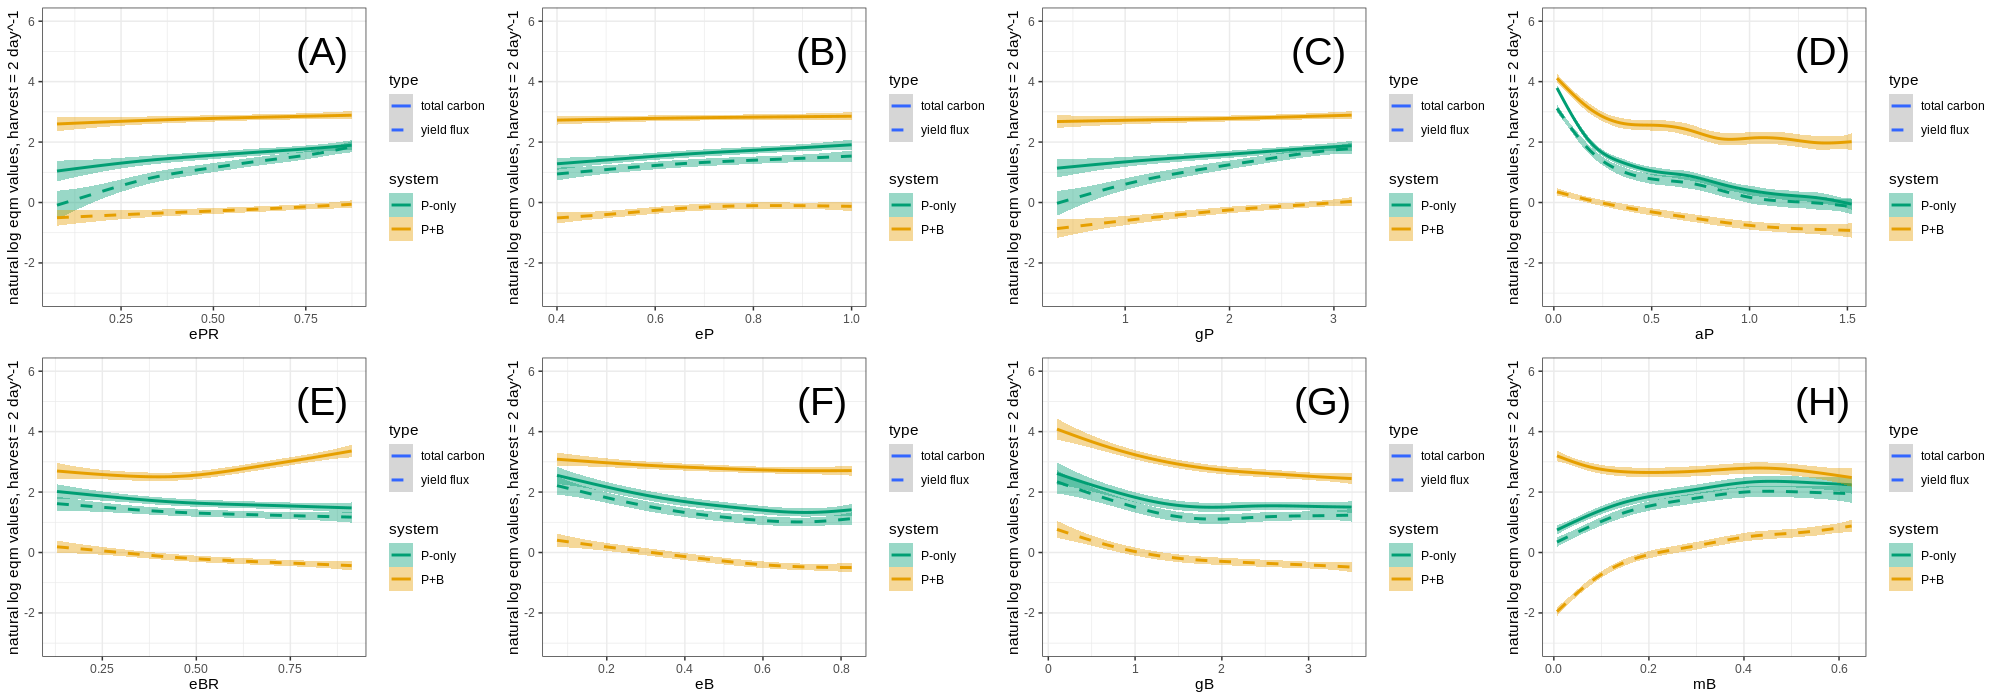
\includegraphics[width=\linewidth]{../result/var_20.png}
    \caption[95\% distribution for $x=2day^{-1}$]{Line graphs showing 95\% confidence interval for ``log total carbon" (solid line) and ``log yield flux" (dash line) based on respective parameter ranges when removal rate = 2$day^{-1}$.  {\scriptsize hi}}
    \label{fig:v10}
\end{figure}

\subsection{total carbon}
\begin{itemize}
    \item 95\% distribution don't overlap between P+B \& P-only systems
    \item highest difference happen in low $g_P$ and lowest difference in low $a_P$ regions respectively
    \item overall distribution (left histogram) has P+B distribution peaked on the right of the P-only one
    \item due to the stability in the P+B result (small 95\% interval on each solid line and across the 8 parameters), peak density of P+B higher than that of P-only
\end{itemize}

\subsection{org-C / yield}
\begin{itemize}
    \item log(yield)|$_{x=1}$ = log(org-C) + log($x$) = log(org-C)
    \item change of P parameters do not have observable effect on P+B log value (in smaller $x$ values fluctuated more)
    \item change of B parameters gave more consistent effect across parameter ranges
    \item most P+B values are higher than that of P-only
    \begin{itemize}
        \item $e_{PR}$, $g_P$, $g_B$ got (close to be) overtaken by P-only distributions
        \item $e_P$, $e_{BR}$, $e_B$ always had their distributions higher than P-only
        \item $a_P$, $m_B$ had P+B overtook P-only values at small parameter values
    \end{itemize}
    \item overall distribution (middle histogram) having P+B higher in central peak density; P-only has a wider spread in log carbon pool size
\end{itemize}

\end{document}
